\documentclass[11pt]{article}

%  USE PACKAGES  ---------------------- 
\usepackage{float}
\usepackage{enumitem}
\setlist[itemize]{noitemsep, topsep=0pt}
\usepackage[margin=0.7in,vmargin=1in]{geometry}
\usepackage{amsmath,amsthm,amsfonts}
\usepackage{amssymb}
\usepackage{fancyhdr}
\usepackage{fancyvrb}
\usepackage{enumerate}
\usepackage[T1]{fontenc}
\usepackage{mathtools}
\usepackage{graphicx}
\usepackage{tcolorbox}
\usepackage{hyperref,color}
\usepackage{enumitem,amssymb}
\newlist{todolist}{itemize}{4}
\setlist[todolist]{label=$\square$}
\usepackage{pifont}
\fvset{fontsize=\small,fontfamily=times}
\newcommand{\cmark}{\ding{51}}%
\newcommand{\xmark}{\ding{55}}%
\newcommand{\done}{\rlap{$\square$}{\raisebox{2pt}{\large\hspace{1pt}\cmark}}%
\hspace{-2.5pt}}
\newcommand{\HREF}[2]{\href{#1}{#2}}
\usepackage{textcomp}
\usepackage{listings}
\lstset{
basicstyle=\small\ttfamily,
% columns=flexible,
upquote=true,
breaklines=true,
showstringspaces=false
}
%  -------------------------------------------- 

%  HEADER AND FOOTER (DO NOT EDIT) ----------------------
\pagestyle{fancy}
\fancyhead{}
\newcommand{\newquestion}[1]{
\clearpage % page break and flush floats
\renewcommand{\problemnumber}{#1} % set problem number for header
\phantom{}  % Put something on the page so it shows
}
\fancyfoot[L]{IE 332}
\fancyfoot[C]{Project Submission}
\fancyfoot[R]{Page \thepage}
\renewcommand{\footrulewidth}{0.4pt}

%  --------------------------------------------


%  COVER SHEET (FILL IN THE TABLE AS INSTRUCTED IN THE ASSIGNMENT) ----------------------
\newcommand{\addcoversheet}{
\clearpage
\thispagestyle{empty}
\vspace*{0.5in}

\begin{center}
\Huge{{\bf IE332 Project \#2}} % <-- replace with correct assignment #

Due: April 28th, 11:59pm EST % <-- replace with correct due date and time
\end{center}

\vspace{0.3in}

\noindent We have {\bf read and understood the assignment instructions}. We certify that the submitted work does not violate any academic misconduct rules, and that it is solely our own work. By listing our names below we acknowledge that any misconduct will result in appropriate consequences. 

\vspace{0.2in}

\noindent {\em ``As a Boilermaker pursuing academic excellence, I pledge to be honest and true in all that I do.
Accountable together -- we are Purdue.''}

\vspace{0.3in}

\begin{table}[h!]
  \begin{center}
    \label{tab:table1}
    \begin{tabular}{c|ccccc|c|c}
      Student & Algorithm & Complexity & Implementation & Testing & Report & Overall & DIFF\\
      \hline
      Matt Fortier & 40 & 20 & 10 & 15 & 15 & 100 & 0\\
      Geoffrey Ladue & 15 & 20 & 10 & 15 & 40 & 100 & 0\\
      Josiah Mann & 15 & 20 & 10 & 40 & 15 & 100 & 0\\
      Anthony Matejko & 15 & 20 & 35 & 15 & 15 & 100 & 0\\
      Shamam Tabindah & 15 & 20 & 35 & 15 & 15 & 100 & 0\\
      \hline
      St Dev & 11 & 0 & 14 & 11 & 11 & 0 & 0
    \end{tabular}
  \end{center}
\end{table}

\vspace{0.2in}

\noindent Date: \today.\\

\noindent \textbf{\href{https://github.com/gladue0427/IE-33200-Project-2}{Public GitHub Repository Link}}
}
%  -----------------------------------------

%  TODO LIST (COMPLETE THE FULL CHECKLIST - USE AS EXAMPLE THE FIRST CHECKED BOXES!) ----------------------


%% LaTeX
% Für alle, die die Schönheit von Wissenschaft anderen zeigen wollen
% For anyone who wants to show the beauty of science to others

%  -----------------------------------------


\begin{document}


\addcoversheet
\pagebreak
\tableofcontents
\pagebreak

\section{Main Text}

\subsection{Algorithms}

\subsubsection{Algorithm 1}

\noindent This R function, find\_most\_green, takes an input image y (represented as a 3-dimensional array with dimensions for height, width, and color channels) and a pixel\_budget parameter, and returns the indices of the pixel\_budget most green pixels in the image.\\

\noindent The function uses the difference between the green channel and the sum of the red and blue channels to calculate the "greenness" of each pixel. This is a common heuristic for identifying green areas in an image. The function sorts the pixels by their greenness and returns the indices of the top pixel\_budget pixels. This approach prioritizes the most green pixels and ignores other information about the image.\\

\noindent The choice of the greenness heuristic is reasonable because it's a quick and easy way to identify green areas in an image. It's not perfect and may miss some green areas, but it's often good enough for simple tasks like this. Sorting the pixels by greenness and returning the top pixel\_budget pixels is an optimal approach because it prioritizes the most green pixels, which is likely to produce the most noticeable visual effect.\\

\noindent The function calculates the greenness of each pixel, which requires iterating over all the pixels in the image. The pixel\_budget parameter can be used to control the number of pixels that are changed. A larger pixel\_budget will result in more noticeable changes to the image, but takes longer to run. This function is not directly related to generating testing pairs for machine learning algorithms, but it could be used as a pre-processing step to modify images before feeding them into a machine learning algorithm.\\

\begin{center}
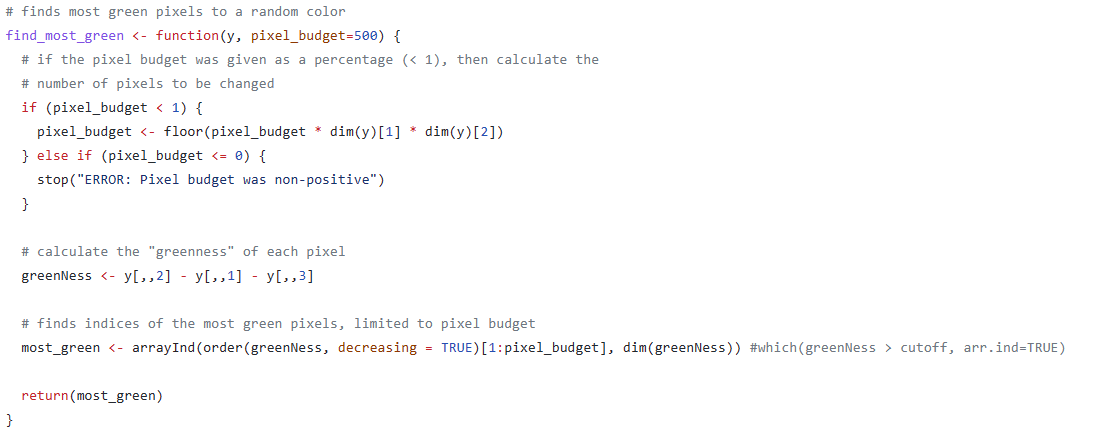
\includegraphics[scale=.75]{Algo1.png}\\
\textbf{Figure 1: Green to Random Algorithm}
\end{center}

\subsubsection{Algorithm 2}

\noindent This code defines a function called "find\_most\_yellow" that takes an input image "y" and a pixel budget as arguments. The function calculates the "yellowness" of each pixel in the image by adding the green and red channels and subtracting the blue, and then finds the indices of the pixels with the highest yellowness values, limited to the specified pixel budget. This algorithm was chosen to specifically target and change the yellow pixels that would be more present in dandelion images.\\

\noindent In terms of design decisions, the use of the "arrayInd" function to convert the linear indices of the most yellow pixels back to their original 2D indices is a good choice as it avoids the need for a nested loop. Additionally, the use of the "order" function to efficiently sort the greenness values in decreasing order was considered to be a quality consideration by the team.\\

\noindent The choice of using the yellowness value as a proxy for "yellowness" is a somewhat simplistic approach, as it doesn't take into account other factors such as saturation or hue that might also contribute to a pixel being perceived as "yellow". However, it may be sufficient for some applications.\\

\noindent Regarding testing pairs for machine learning algorithms, this function does not generate testing pairs for machine learning algorithms directly, as it is only concerned with finding the most yellow pixels in an image. However, the output of this function could potentially be used as input to a machine learning algorithm as a way of identifying regions of interest in an image.\\
\begin{center}
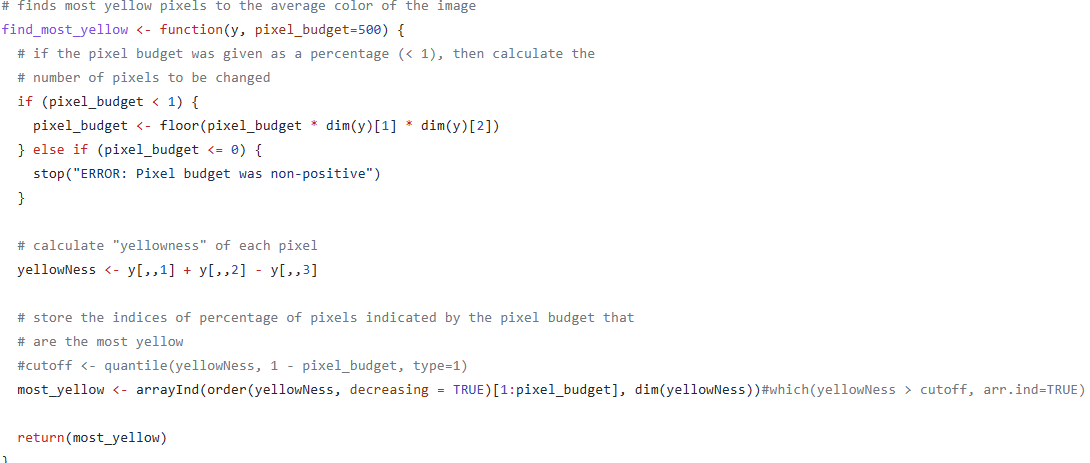
\includegraphics[scale=.75]{Algo2.png}\\
\textbf{Figure 2: Average Yellow Algorithm}
\end{center}

\subsubsection{Algorithm 3}

\noindent This function is designed to find random pixels in an image for modification and takes two arguments: the image data as a matrix y and the pixel budget pixel\_budget as an integer or a percentage. The pixel budget is the maximum number of pixels that can be changed in the image. This algorithm can be used to make a color either more or less prevalent throughout the image\\

\noindent  The function initializes a matrix change\_pixels to store the row and column indices of the pixels to be changed. The number of rows in change\_pixels is equal to the pixel budget. It then generates random row and column indices using the runif function and stores them in change\_pixels. The function returns the matrix change\_pixels.\\

\noindent To generate testing pairs for a machine learning algorithm using this function, one could use the original image as the input and the output image as the expected output. The machine learning algorithm would then be trained to learn the mapping between the input image and the output image.\\

\begin{center}
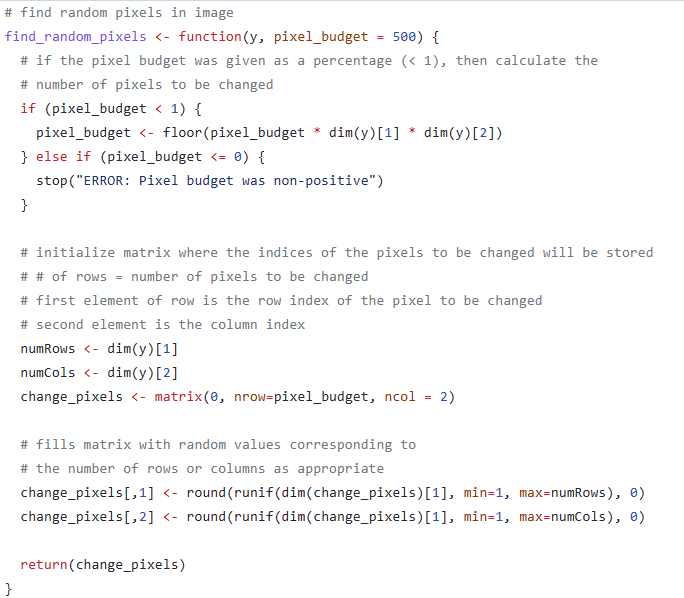
\includegraphics[scale=.75]{Algo3.png}\\
\textbf{Figure 3: Random Pixel Algorithm}
\end{center}


\subsubsection{Algorithm 4}

\noindent This code finds the most average pixels in an image. It takes in an image y and a pixel budget pixel\_budget as input, and returns the indices of the most average pixels limited to the pixel budget. This purpose of this algorithm was to replace the most average pixels with either random colors to increase the color variability in the image or shift the mean value in a desired direction, which could be useful for fooling the classifier.\\

\noindent First, the mean value of each color channels in the image is calculated using R's built-in mean() function. Next, the distance of each pixel's color from the average image color is calculated. The code uses the Manhattan distance formula to calculate the distance, which is the sum of the absolute differences of each color value from the mean.\\

\noindent Finally, the code uses the arrayInd() function to find the indices of the most average pixels. This function returns the indices of the elements in a flattened array that correspond to a given set of subscripts. This is a reasonable decision as it allows for easy indexing of the image matrix.\\

\noindent For testing pairs in machine learning algorithms, the output of this function could be used as a mask to change the color of the most average pixels. The knowledge representation in this case would be the indices of the most average pixels, as this is all that is needed to modify the image.\\

\begin{center}
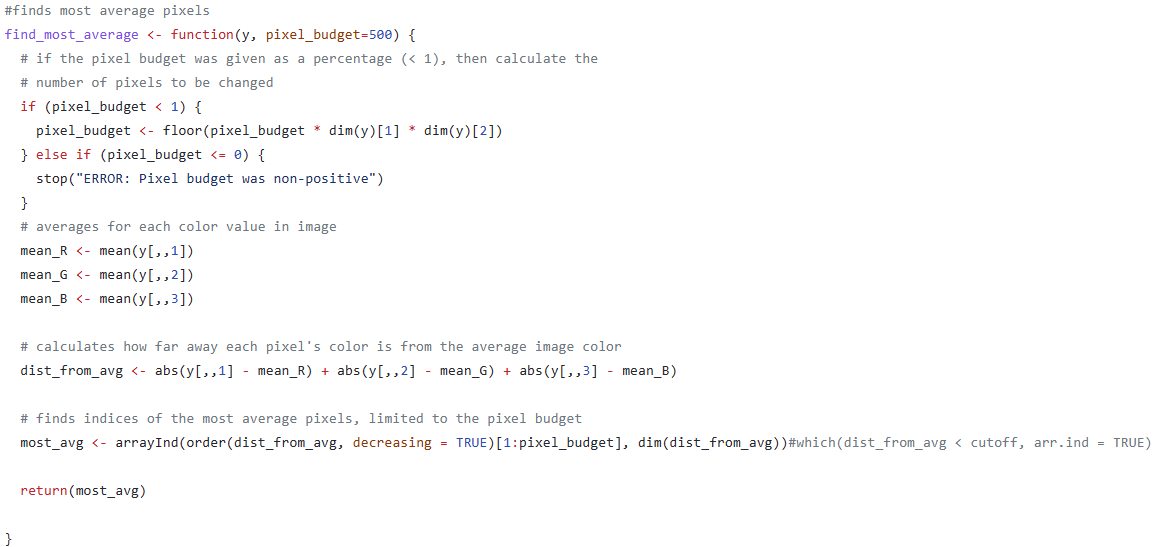
\includegraphics[scale=.75]{Algo4.png}\\
\textbf{Figure 4: Most Average Pixel Algorithm}
\end{center}

\subsubsection{Algorithm 5}

\noindent This function find\_least\_average takes an image array y and a pixel\_budget as input and returns the indices of the least average color pixels out of the image. This algorithm has the same structure as find\_most\_average, but it returns the pixels with color values furthest away from the average color instead of the closest. This was done because the team reasoned that pixel values further away from the mean value would have a larger effect on the classifier, and removing this effect could potentially change its outcome.\\

\noindent To generate testing pairs for machine learning algorithms, the function can be used to select a certain number of pixels with the least average color and then these pixels can be changed by a certain amount to generate the test image pairs.\\

\begin{center}
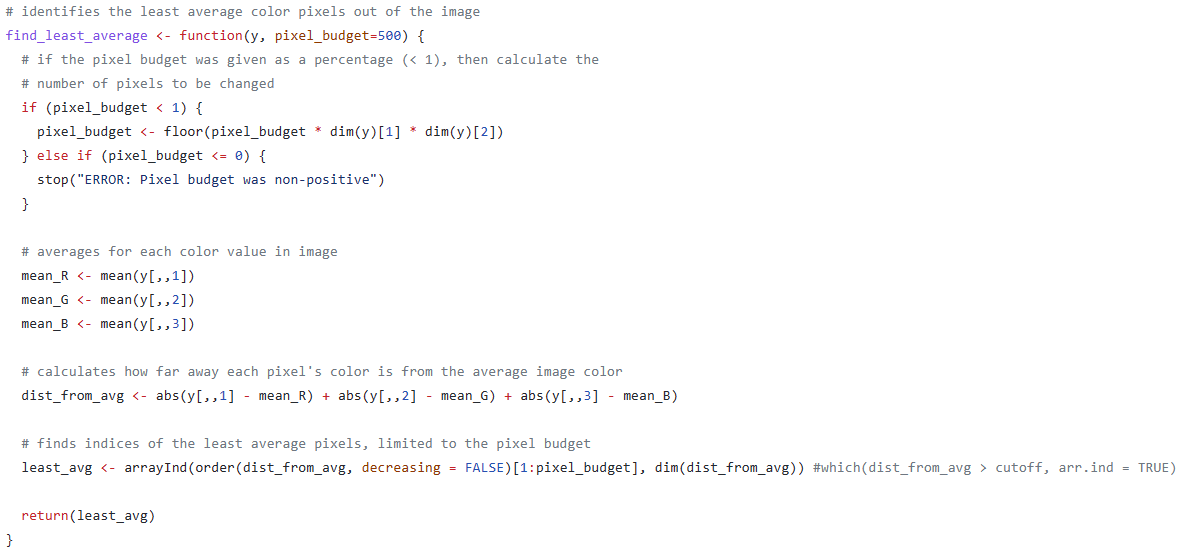
\includegraphics[scale=.75]{Algo5.png}\\
\textbf{Figure 5: Least Average Pixel Algorithm}
\end{center}

\subsubsection{Weighted Algorithm}

\begin{center}
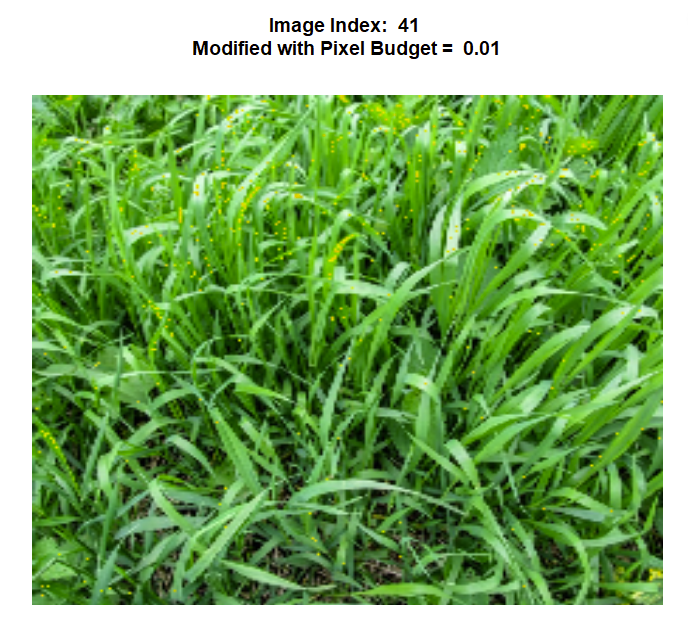
\includegraphics[scale=.75]{GrassMod.png}\\
\textbf{Figure 6: Modified Grass Image}
\end{center}

\begin{center}
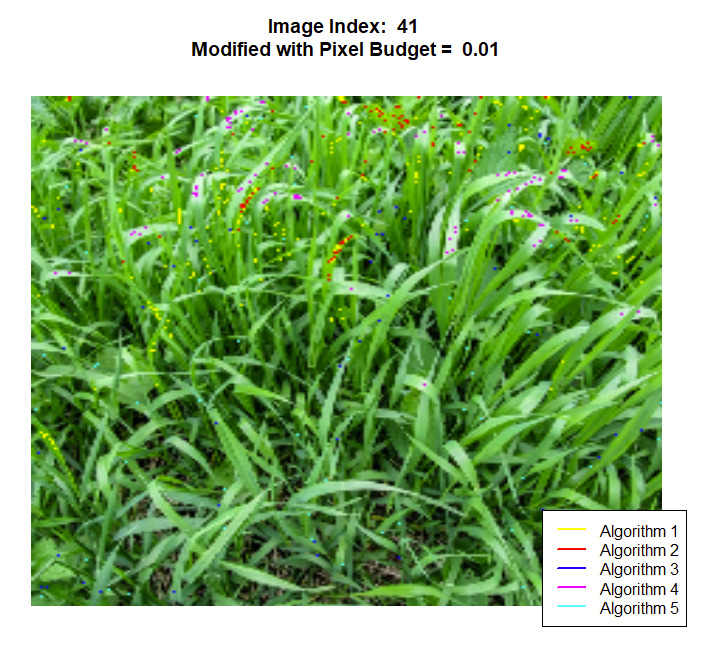
\includegraphics[scale=.75]{GrassModCol.png}\\
\textbf{Figure 7: Color Coded Grass Image}
\end{center}

\begin{center}
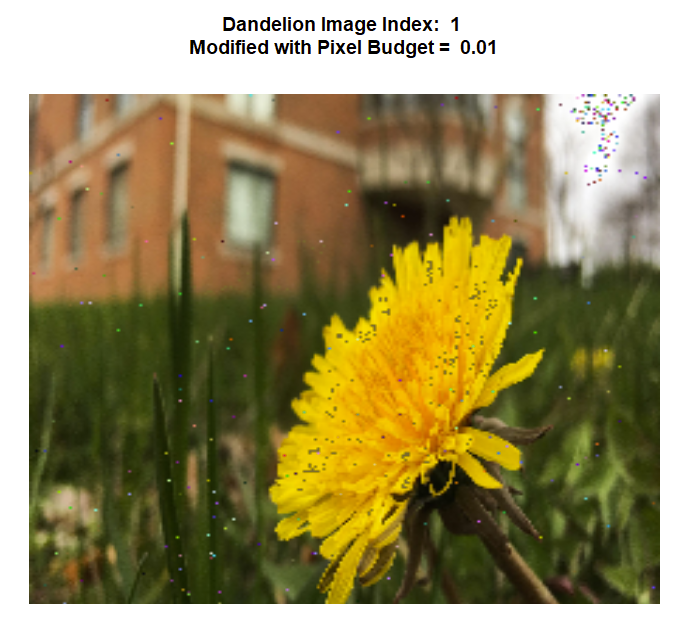
\includegraphics[scale=.75]{DanMod.png}\\
\textbf{Figure 8: Modified Dandelion Image}
\end{center}

\begin{center}
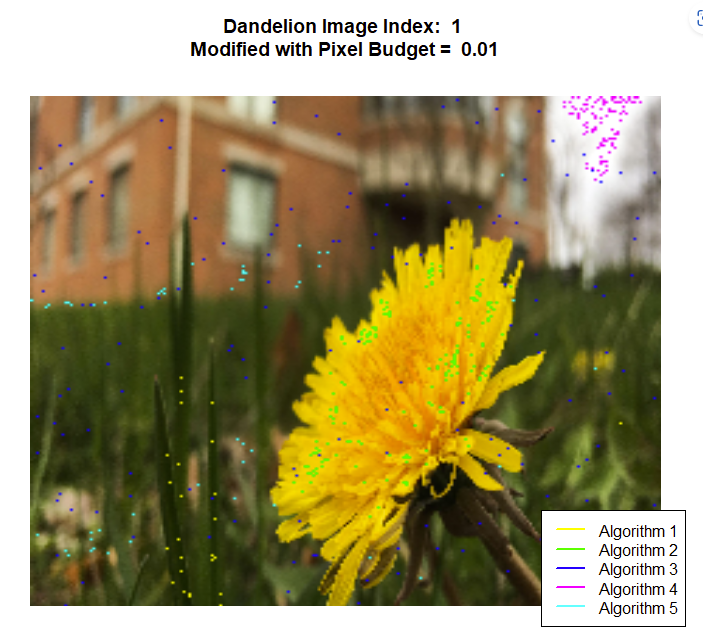
\includegraphics[scale=.75]{DanModCol.png}\\
\textbf{Figure 9: Color Coded Dandelion Image}
\end{center}

\noindent Based on Figures 7 \& 9, the color coded grass and dandelion images, respectively, pixels selected by each algorithm are consistent with their expected output. The weighted algorithm takes each of the five formative methods and assigns weights to each. This is done to determine how many pixels to choose from each algorithm in order to change the final outputted image. A more advanced and optimal manner of assigning weights is discussed in Section 1.2.6, in which a machine learning-based algorithm would have selected the best implementation out of the possible alternative algorithms the team engineered.\\

\noindent The mod\_image() function is designed to modify a 3-layer matrix that represents an image, transforming it to either resemble grass or a dandelion, as seen in the above figures. This is achieved by changing some of the original image's pixels to a realistic shade of yellow resembling a dandelion.\\

\noindent The function takes three arguments: y, a 3-layer matrix that represents the original image; pixel\_budget, which is amount of pixels to be changed as either a percentage or the absolute number; and type, which specifies whether the original image represents grass or a dandelion, corresponding to a 0 or 1 respectively.

\noindent Before processing the image, the function checks the validity of the pixel\_budget argument. If it is non-numeric or NA, an error is thrown. If it is less than or equal to zero, or greater than the total number of pixels in the image, an error is also thrown. If the value of pixel\_budget is less than one, it is converted to the corresponding absolute number of pixels to change.\\

\noindent The function then sets the seed for the random number generator to ensure it is reproducible, calculates the mean values of the red, green, and blue color layers of the original image, and proceeds to call the five sub-algorithms that identify the pixels to change. These include find\_most\_green(), find\_most\_yellow(), find\_random\_pixels(), find\_most\_average(), and find\_least\_average(). Each of these functions is designed to identify a specific subset of pixels within the image, limited by the value of the pixel\_budget argument.\\

\noindent Following this, the function sets weights for each algorithm that will change the pixels, and calculates the number of pixels each algorithm will change based on the pixel\_budget.\\

\noindent The function then modifies the identified pixels, based on the type of the input image, by changing the most green pixels, most yellow pixels, random pixels, most average, and least average pixels. For grass images, all pixels are changed to a shade of yellow that could be expected in the petals of a dandelion, which was done in an attempt to have the classifier ``think'' a dandelion was in the image. For dandelion images, the most yellow pixels are changed to the average color in the image, while all other selections of pixels are changed to random colors. This was done with the intention of reducing the recognizability of the dandelion while also adding random noise. Lastly, the function returns the modified image matrix.\\

\noindent The mod\_image() function is a useful tool for image manipulation, offering flexibility and control over the transformation process, and its well-structured design ensures efficient processing.

\subsection{Extended Research \& Attempted Methods}

\noindent Although we implemented the algorithms outlined in Section 1.1, the team devoted significant time to researching common methods of adversarial attacks and even generated corresponding alternatives in R. These attempted methods, while unsuccessful upon implementation, are a worthwhile case study in the team's product development.

\subsubsection{Random Pixel Flip}

\noindent Random pixel flipping generates perturbed images that can be used to confuse a machine learning model. The idea behind this technique is to flip the value of one or more pixels in an image to create a new image that is similar to the original image but that the machine learning model will classify differently.\\

\noindent From the team's research, the main advantage of random pixel flipping is that it is a simple and efficient way to generate a large number of adversarial examples quickly. By randomly flipping a small number of pixels in an image, the algorithm can generate many different perturbed images that are all slightly different but still belong to the same class. This makes it difficult for the machine learning model to distinguish between the original image and the perturbed images.\\

\noindent The team's rough outline of this particular method works by first calculating the number of pixels to flip based on the image dimensions and the budget specified by the user. It then generates a set of perturbed images by randomly flipping the specified number of pixels in the original image.\\

\noindent Finally, the algorithm counts the number of occurrences of each class among the perturbed images and returns the most common class. This allows the algorithm to determine which class the machine learning model is most likely to predict for the perturbed images, even though they are all slightly different from the original image.\\

\noindent Overall, random pixel flipping can be a useful tool for adversarial attacks because it allows an attacker to generate a large number of perturbed images quickly and efficiently, making it difficult for a machine learning model to accurately classify the images. This can be particularly useful in situations where an attacker wants to trick a machine learning model into making a specific prediction.

\subsubsection{Decision Trees}

\noindent The team also researched Random Forest algorithms in depth to determine if it would be suitable to explore decision tree-based solutions. The code outlined by the team could have been a powerful tool for adversarial tasks if paired with methods of modifying pixels. The use of parallel processing helps to speed up the computation time, allowing for faster model training and permits the model to train sample data and learn patterns within it. Once the model is trained based various image modification techniques, it can combine them to optimally fool the given classifier. This makes it a useful tool for adversarial attacks, as it can be used to identify vulnerabilities in image classification systems and create adversarial images.

\subsubsection{Stack Generalization}

\noindent The ensemble learning method developed by the team would have been utilized for the purpose of adversarial attacks as it combines multiple models to improve the accuracy of the classifier, which can make it more robust against adversarial attacks. The base learners used in this code, including a decision tree, a naive Bayes classifier, and a random forest, were combined through the team's research since they are known to be susceptible to adversarial attacks. By combining them in an ensemble, the resulting model may be less vulnerable to such attacks. Additionally, by using the validation set to evaluate the performance of the model, the code can identify potential weaknesses or vulnerabilities in the model, which can be used to improve its robustness against adversarial attacks. While this method was unsuccessful, this was the team's attempt to integrate multiple algorithm methods.

\subsubsection{Fast Gradient Sign Method}

\noindent A Fast Gradient Sign Method (FGSM) attack was attempted based on its widespread use and proven effectiveness during the team's research.\\

\noindent The FGSM would use the Keras and Tensorflow libraries to generate an adversarial image using the pre-trained model, input image, target label, and epsilon value, which determines the degree of change to the original pixal colors. The functions available in the Tensorflow library would be used to obtain the loss function and gradient of the given model. These parameters are then used to produce a set of perturbations that, when added to the original image, would fool the classifier.\\ 

\noindent The epsilon value could be determined through manually testing different values, but ideally a separate machine learning algorithm would be used to find an optimal value or set of values to use. Due to the limitation of a pixel budget and the fact that the final color of a modified pixel is irrelevant, epsilon values could be larger than what is typically used.\\

\noindent The team attempted to implement this strategy, but many challenges were encountered that led to the decision to not continue with it. Although documentation was available for the functions used in an FGSM attack, it was written for Python and used the ``tensor'' data type for all inputs and outputs. Translating the documented Python functions to R and converting the variables used within them to tensors proved to be very challenging, and was determined infeasible with the team's available time and resources. Even though it was not ultimately used, the FGSM attack would have likely been an effective method of performing the task at hand.

\subsubsection{Alternative Weighting Method}

\noindent As outlined throughout Section 1.2, the team researched potential methods for adversarial attack implementation. In addition to these strategies, a method of weighting the outputs of the five sub-algorithms would be necessary. The colors of pixels in the given images are not independent, as pixels are likely to have a similar color to neighboring pixels. Thus, a decision tree based on Bayes' Theorem would not be used. Ideally, a Convolution Neural Network (CNN) would be used, as it is commonly used for image analysis and can identify the underlying identifying characteristics of an image.\\

\noindent The network would be trained to combine the output of the sub-algorithms' output in a way that produces the inverse outcome of the given classifier. However, the network would have to consider all combinations of image modifications during training, so it would likely be highly computationally intensive. Thus, the configuration of the CNN would initially be simple, with one layer and a few nodes. Then, the complexity of the network would gradually be increased, until either the training time is excessively long or over-fitting occurs. The resulting model would be capable of optimally weighing the sub-algorithms for any input image.

\pagebreak

\section{Appendices}

\subsection{Testing / Correctness / Verification}

\noindent Extensive testing was performed on each of the sub-algorithms used to modify the images, themselves, in order to verify that the main model functioned properly. Our group's approach to verifying the correctness of each sub-algorithm consisted of running each program with varying pixel budgets to ensure that we received the image that was modified to the extent specified by the pixel budget. After running each sub-algorithm, we were able to conclude that each sub-algorithm modified the images as expected. It is worth noting that this was done for pixel budgets of one, five, ten, and twelve percent and the difference in pixel budget input had a noticeable difference in the extent to which the image was modified.\\

\noindent Testing was also performed on our main algorithm as well to verify that it too produced our intended results. As with the testing of individual sub-algorithms, we wanted to ensure that the images being passed to the main algorithm were being modified. This result indicated that both images of grass and dandelions were able to be modified.\\

\noindent After checking to ensure that our main algorithm was at the very least functional, we desired to guard against invalid inputs for the pixel budget. Consequently, we added "if" statements with nested "stop" commands to ensure that the pixel budget being passed to the function was not negative, null, NA, non-numeric, or exceeding the total number of pixels in the image (see Figure 10). We then tested the robustness of the program by providing inputs for each of the previously listed cases. This test was also successful.\\

\begin{center}
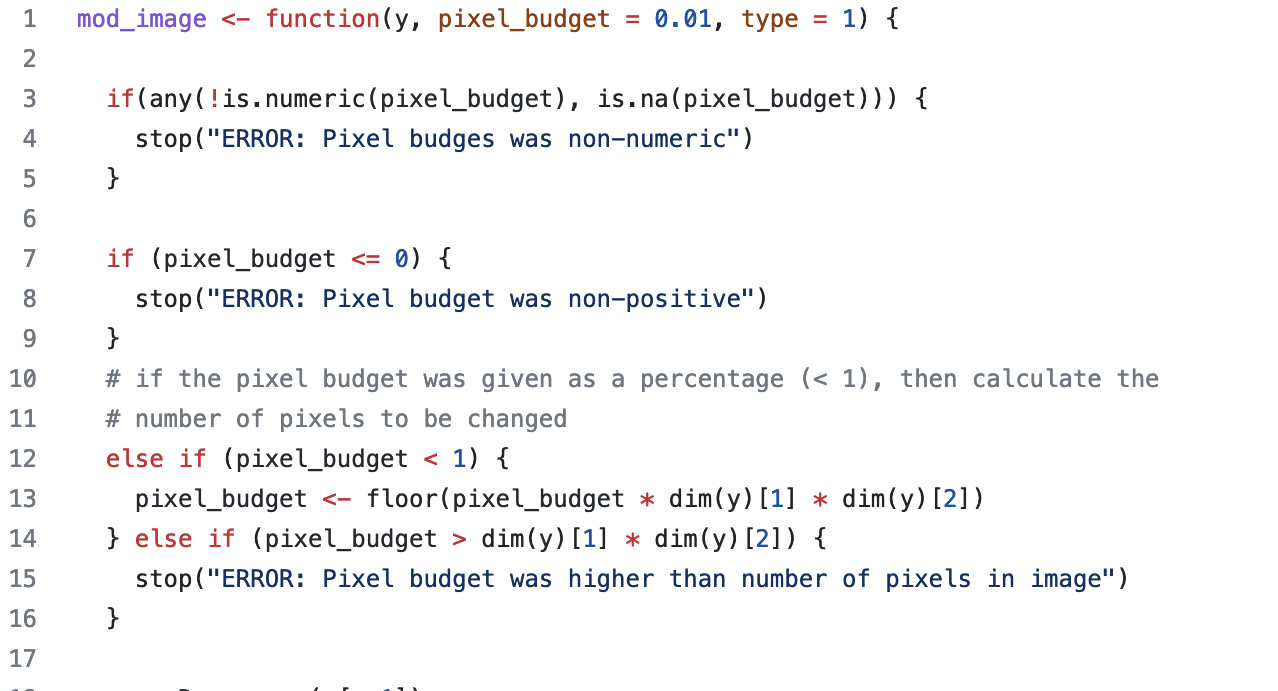
\includegraphics[scale=.75]{Project2.png}
\textbf{Figure 10: Input Verification of Pixel Budgets}
\end{center}

\noindent It is worth noting that while our testing initially began by using grass images to fool the image classifier, we were unable to achieve much success despite the images clearly being unrecognizable. We were, however, able to attain our desired results using the dandelion images. Consequently, we decided to continue using dandelion images rather than grass for the remainder of the project. \\

\noindent While our first successful test run to verify the accuracy of the main algorithm when collaborating with the image classifier fooled the classifier for only 3 out of the 38 dandelion images using a one percent pixel change, we were ultimately able to fool the classifier for 7 out of the 38 images with the same pixel budget. This increase in performance was achieved by ensuring that our main algorithm changed pixels in the image using each sub-algorithm independently, rather than each sub-algorithm successively changing the image output by the previous sub-algorithm. This increase can also be attributed to restricting the algorithm from restricting any images that were passed to the function.\\

\noindent It was observed that when the pixel budget fails to be sufficiently high enough, no changes are actually made to the image. In general, it was also observed that the number of pixels changed in the image are lower than what is specified in the pixel budget. This is due to rounding performed when determining the weighted number of pixels to change from each sub-algorithms' output.


\subsection{Run-time Complexity and Wall-time}

\noindent When it comes to run-time complexity, each sub-algorithm, except for Algorithm 3, call the order() function, which, according to R's documentation, uses a shell sort algorithm. This function is an efficient way to sort elements of an array. The run-time complexity of this algorithm can depend on our choice of gap sequence and the data that we input. The shell sort algorithm has, in our case, a run-time complexity of O($p^{4/3}$), with $p$ being the total number of pixels. Each sub-algorithm that uses the order() function would have a run-time complexity of O($p^{4/3}+b$), with $b$ being the pixel budget, as each algorithm selects $b$ pixels. Algorithm 3's run-time would simply be O($b$), as it only uses R's build in function to generate coordinates for b pixels. The total run-time of the weighted selection algorithm would be O($4*(p^{4/3}+b)+2b$), as all four sub-algorithms calling order() are run along with Algorithm 3, and then a total of $b$ pixels are chosen to be changed from the selections of each of the sub-algorithms . These grow to the power of 4/3 the size of input. With this run-time complexity, the larger the input, the slower the algorithm will work.\\

\begin{center}
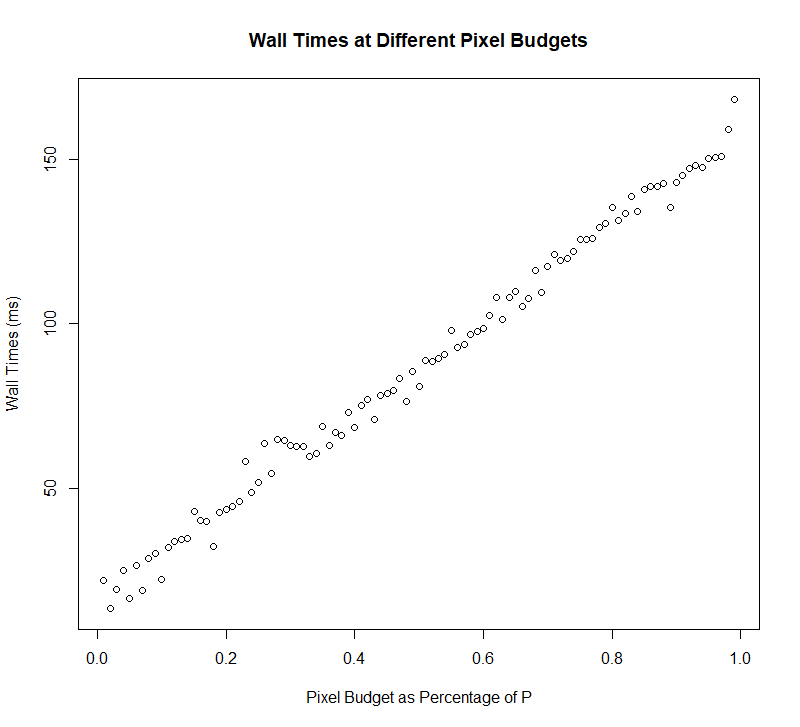
\includegraphics[scale=.6]{WallTimes.png}\\
\textbf{Figure 11: Wall Times at Different Pixel Budgets}
\end{center}

\noindent In regards to our algorithms wall-time, we can see that there is a linear relationship between the increase in pixel budget and wall-time. As we continue to increase the pixel budget, $b$, from our run-time complexity equation above, we can see through the graph that the wall-time is increasing in a linear relationship. 

\subsection{Performance}
To calculate performance score, the following formula is used. In this formula, P represents the total number of pixels in the image and f denotes the number of successfully fooled images at a given budget level b.\\
$$ \qquad \sum_{b=1}^{0.01*P} f*P/b $$ 
After resizing all the images, the value of P was calculated as 224*224 =50176. which means that the budget level ranges from 1 up to approximately 502 (i.e., 0.01*P = 501.76). \\
The total performance score of the algorithm used to fool the model with dandelions was determined to be 284,458.249. Moreover, it is worth noting that the lowest budget required to fool an image was when\\ b = 3 for image ``dandelionflowerrib-1878096549.jpg''.\\
The algorithm performance score to fool the model with grass was determined to be 0 as there were no successfully fooled images at any budget level.\\ 

\begin{center}
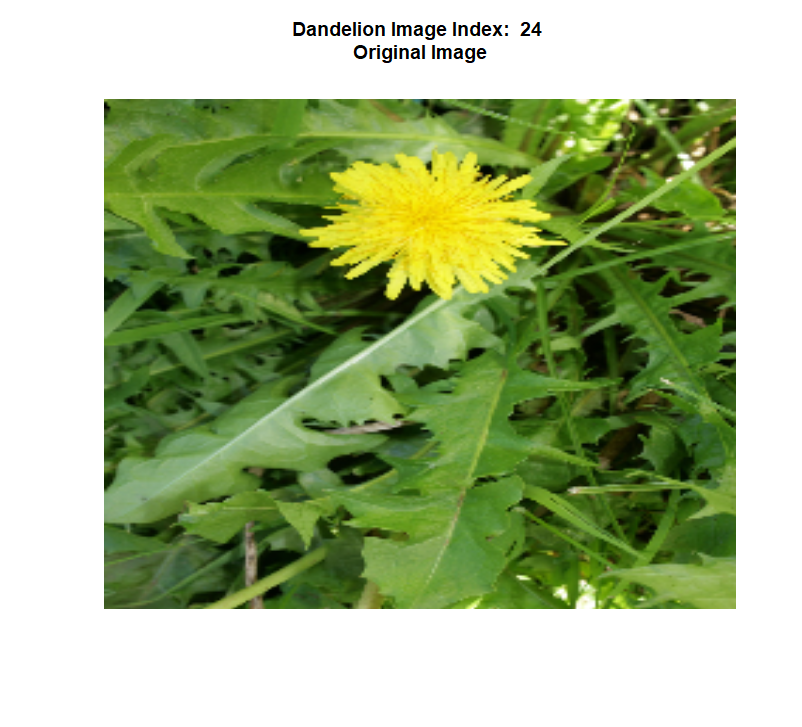
\includegraphics[scale=.42]{dandelion_original.png}
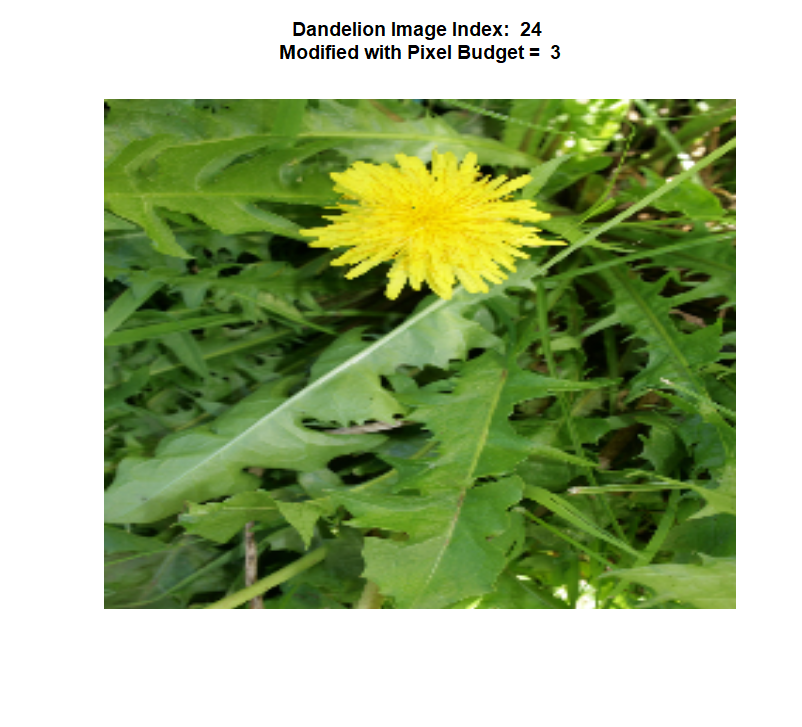
\includegraphics[scale=.42]{dandelion_modified.png}\\
\textbf{Figure 12: Lowest Budget Level required to Fool a Classifier}
\end{center}

\subsection{Justification}

\noindent Although machine learning methods were not used in the final implementation of the main and sub-algorithms, the chosen methods of selecting and changing pixels were not chosen arbitrarily. They were instead based on the context of the types of images used and the given classifier model. For example, dandelion images have their most yellow pixels changed to the average color of the image while pixels chosen with through different methods are changed to a random color. This was done in order to reduce any features that the classifier would recognize as a dandelion while also adding random noise. Ultimately, the methods used were a manual, simplified implementation of the longer and more optimal process that machine learning algorithms would use to perform the same task. Despite the simplistic justification for the team's final product, the technical description of each algorithm and their corresponding design considerations, run-time vs. performance metrics, and limitations are outlined in Section 1.1 and provide evidence of their usability; however, the implementation reasoning for these algorithms differed greatly from those detailed in Section 1.2.\\

\noindent It is important to recognize the team's due diligence in researching and even engineering several intricate algorithms, which were detailed in Section 1.2. While the team's final implementation was chosen primarily based off the algorithms' feasibility, attempts were made to implement machine-learning based solutions that would have selected a "one best method," or at least diverged from a more brute force approach. The reason that these alternative solutions could not be implemented can be assigned to the complexity of these methods; however, the technical details and reasoning behind the validity of these approaches (refer to Section 1.2) led to the formation of the final grouping of algorithms outlined earlier in this section. Overall, the team's research-driven approach would not have been as successful without the exploration of aforementioned neural networks.
\end{document}